\documentclass[12pt, letterpaper]{report}
\usepackage[utf8]{inputenc}
\usepackage{graphicx}
\usepackage{indentfirst}

\graphicspath{{./images/}}

\begin{document}

\tableofcontents
\clearpage
%- Requirements
%	Problem Statement
%	Constraints
%	Requirements
%	HW and SW Specification
%	Analysis Verification
\chapter{Introduction}
\section{Problem Statement}
Due to COVID-19 [ref], many countries established mandatory lockdown, which increased the usage of entertainment platforms. Television continues to have an important role in this matter, and that’s why a better user experience, through a good interface, is increasingly needed.
Despite knowing that smart TV’s market is growing, because of its features, a large percentage of the televisions in use are non-smart TV’s [ref], which use infrared sensors to allow the user to control the TV, via a remote control. In this report, it will be analyzed and designed a remote control with the following characteristics: it must control the TV using an infrared sensor, it must be light and battery powered. It should have three buttons: one to switch the TV on/off, called “Power”; the other two buttons are used to scroll up/down and select the available channels, and they are labeled with the arrows up/down, respectively. The main goal of this project is to consolidate the methods of the Waterfall model, as it is a classic model in software development methodology, suitable for small-scale projects.

\section{Problem Statement Analysis}
In order to have a better and deeper understanding of the problem, it’s essential to identify the entities involved and their relationships. Using that analysis, a system diagram can be built, figure \ref{fig:prob_statement}, relating the known entities and presenting some attributes.

\begin{figure}[ht]
	\centering
	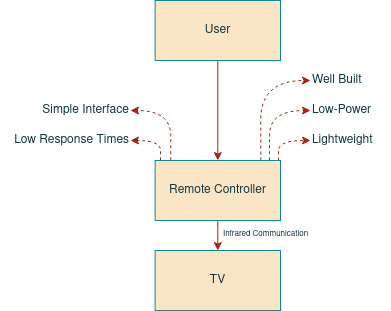
\includegraphics[width=0.75\textwidth]{prob_statement}
	\caption{Problem Statement Analysis Diagram.}
	\label{fig:prob_statement}
\end{figure}

This image, figure \ref{fig:prob_statement}, shows that the remote controller is the only interface between the user and the TV. The user interacts with the remote by pressing one of the existing buttons, and in turn, the remote interacts with the television via an infrared beam. Knowing that the remote controller must have a long lifespan, it must be well built, in order to resist eventual falls, and also, it must have a low consumption, in order to avoid the frequent change of batteries. For a better user experience, the remote should be lightweight, have a simple interface and respond quickly to user commands.

\chapter{Analysis}
\section{Market Research}
\subsection{Market Definition}
A remote control, by definition, is an electronic device used to operate another device from a distance, usually wirelessly. These allow you to control different types of devices, such as televisions, air conditioning, DVD players, sound systems, among others. Remote controllers have different technologies to communicate with the devices they control, such as Bluetooth, Wi-Fi, Radio Frequency (RF) and Infrared (IR), the latter being the most used technology in remote controls.

There are three types of remotes:

\begin{itemize}
	\item Dedicated Remote: a remote programmed to control one or more 					specific devices; 

	\item Universal Remote Control: also called a ‘library’ remote, it’s 				programmed by manufacture to control almost all common home devices;

	\item Programmable Remote Control: can be programmed either with codes 				to control devices or create more elaborate functions via a 					computer or mobile app, using USB communication, Bluetooth or Wifi.
\end{itemize}

Regarding the application field, since this allows the operation of devices that are out of convenient reach for direct operation of controls, they may be used in different fields, like industry, civil, military, space, and others.

\subsection{Bench-Marking}
Most of the time, when you buy a device that requires a remote control, it's already included. In the table below, table \ref{table:popular_remotes}, there are shown some of the most popular remotes in the market right now.

\begin{table}[h]
	\centering
	\begin{tabular}{||c c c c c||} 
	\hline
	Product Name & Price (€) & Weight (g) & Comm. Technology & Remote Type\\
	\hline\hline
	Roku Voice & 17,30 & 90,72 & Wi-Fi & Dedicated\\ 
	Apple TV & 25,00 & 18,14 & Wi-Fi, Bluetooth & Dedicated \\
	DIRECTV RC73 & 6,05 & 90,71 & IR, RF & Programmable\\
	IR-1316 & 12,97 & 49,89 & IR & Universal\\
	\hline
\end{tabular}
				
\caption{Most popular Amazon's remote controllers. }
\label{table:popular_remotes}
\end{table}
		
\section{System}
\subsection{System Overview}
As shown in figure \ref{fig:sys_overview}, the push buttons on the remote behave as sensors, which produce an electrical signal whenever they are pressed. This electrical signal is processed by the controller, transmitting to the infrared emitter (actuator) a signal identifying the operation performed by the user, which must be received by the television in order to execute the desired operation.

\begin{figure}[ht]
	\centering
	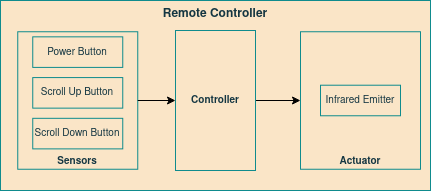
\includegraphics[width=0.75\textwidth]{SysOverview}
	\caption{System Overview Diagram.}
	\label{fig:sys_overview}
\end{figure}

\subsection{System Requirements and Constraints}

Functional Requirements:

\begin{itemize}
	\item Three push buttons: Power button, scroll up button, scroll down button.\\
\end{itemize}

Non-Functional Requirements:
\begin{itemize}
	\item Lightweight;
	\item Low-Power consumption;
	\item Well built;
	\item Simple interface;
	\item Low response times.\\
\end{itemize}

System Constraints:
\begin{itemize}
	\item Time constraint;
	\item 2 Members team;
	\item Infrared communication.\\
\end{itemize}
\section{System Architecture}
A system architecture is the conceptual model that describes the system, based on its structure and behavior. In this way, the system must be described in two ways: hardware architecture, which describes the existing connections between hardware components, and software architecture, which describes the flow of information in the system.

\subsection{Hardware Architecture}
The core of this system is the integrated circuit, which reads the data from the sensors (push buttons) and produces an electrical signal that identifies the operation carried out by the user. This signal is transmitted to the infrared emitter, which converts it into a light signal (infrared). The system's batteries allow powering all components. In figure \ref{fig:hw_arch} it is possible to identify all the hardware components that make up the system. 

\begin{figure}[ht]
	\centering
	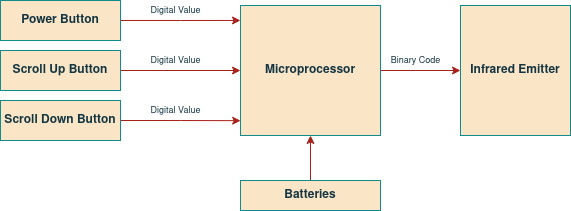
\includegraphics[width=0.75\textwidth]{HW_Arch}
	\caption{Hardware Architecture Scheme.}
	\label{fig:hw_arch}
\end{figure}

\subsection{Software Architecture}


\section{Use Case}

\begin{figure}[ht]
	\centering
	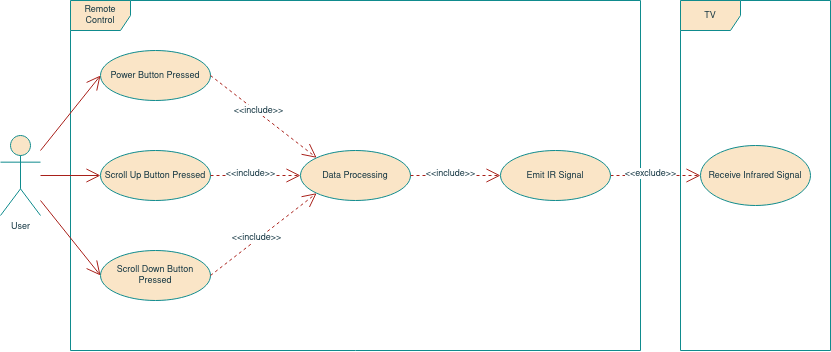
\includegraphics[width=0.75\textwidth]{Use-Case}
	\caption{Use Case Diagram.}
	\label{fig:use_case}
\end{figure}

A use case diagram is a graphical representation of all user’s possible interactions. As shown in figure \ref{fig:use_case}, the user is the only system entity, who can press any of the remote controller buttons. This action triggers the reading of the buttons, producing the respective code related to the pressed button, which is transmitted to the infrared emitter. The television must receive this code, performing the action required by the user.

\section{Sequence Diagram}
A sequence diagram is another graphical representation that describes how and in what order a group of objects interacts. Figure \ref{fig:seq_diagram} shows that a sequence is started when the user presses a button on the remote control. At that moment, the integrated circuit determines which button was pressed, transmitting the respective button code to the infrared emitter. In turn, the infrared emitter emits the button code via an infrared signal.

\begin{figure}[ht]
	\centering
	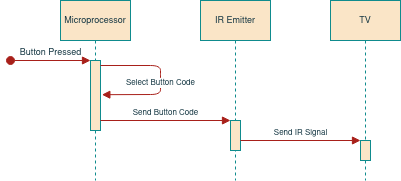
\includegraphics[width=0.75\textwidth]{SequeceDiagram}
	\caption{Sequence Diagram.}
	\label{fig:seq_diagram}
\end{figure}

%- Design
%	Analysis Review
%	HW Components Specification
%	Defining HW interface
%	SW Components Specification
%	Defining SW interface
%	Start-up/shutdown process Specification
%	Errors Handling Specification
%	Design Verification
\chapter{Design}
\section{Hardware Specification}
% microp
% IR emitter
% Resistors
% Buttons
% Batteries
In this section it will be specified the chosen hardware and the presented the interface between each of the components.

\subsection{Microprocessor}
The integrated circuit that will control the operating status of the remote will be the ATtiny85 [ref] (figure FIGURE). This is a well known microcontroller due to its small dimensions, associated capabilities and its low price. Its a good fit for this system because of its low operating voltage and of its ability to read the data given by the sensors, the remote buttons, and produce an adequate response.

\begin{itemize}
	\item Operating Supply Voltage: 1.8V to 5.5V
	\item 8 bit Microcontroller
	\item 8 pins, 6 GPIO pins;
	\item 8 kB of program memory size;
	\item 512 B data RAM size;
\end{itemize}

[FIGURE]


For programming the ATtiny85 it can be used an Arduino board, like Arduino UNO board [ref], which is a one-time process.

\subsection{IR Emitter}
The system’s actuator is an infrared emitter, which has been used in remote controls since the early 1980s. IR sensors are used to measure and detect infrared radiation in its surrounding environment. An IR emitter can be easily found, having the appearence represented in the figure [ref].

[FIGURE]

\subsection{Resistors}
It is known that a light emitting diode (LED), like the IR emitter presented above, admits a maximum forward current. To do that, and as well as to control how much current flows through the remote button’s circuit, it may be used some resistors.

\subsection{Buttons}
??

\subsection{Batteries}
In order to supply the system components, focusing on the microprocessor operating supply voltage, the system may be supplied by two or three batteries AAA, having in mind that each of this batteries works within the range 0.9 V to 1.5 V.

\section{Software Specification}
% Sw used
% Flowcharts

\section{Flowcharts}

\end{document}